\documentclass[1p]{elsarticle_modified}
%\bibliographystyle{elsarticle-num}

%\usepackage[colorlinks]{hyperref}
%\usepackage{abbrmath_seonhwa} %\Abb, \Ascr, \Acal ,\Abf, \Afrak
\usepackage{amsfonts}
\usepackage{amssymb}
\usepackage{amsmath}
\usepackage{amsthm}
\usepackage{scalefnt}
\usepackage{amsbsy}
\usepackage{kotex}
\usepackage{caption}
\usepackage{subfig}
\usepackage{color}
\usepackage{graphicx}
\usepackage{xcolor} %% white, black, red, green, blue, cyan, magenta, yellow
\usepackage{float}
\usepackage{setspace}
\usepackage{hyperref}

\usepackage{tikz}
\usetikzlibrary{arrows}

\usepackage{multirow}
\usepackage{array} % fixed length table
\usepackage{hhline}

%%%%%%%%%%%%%%%%%%%%%
\makeatletter
\renewcommand*\env@matrix[1][\arraystretch]{%
	\edef\arraystretch{#1}%
	\hskip -\arraycolsep
	\let\@ifnextchar\new@ifnextchar
	\array{*\c@MaxMatrixCols c}}
\makeatother %https://tex.stackexchange.com/questions/14071/how-can-i-increase-the-line-spacing-in-a-matrix
%%%%%%%%%%%%%%%

\usepackage[normalem]{ulem}

\newcommand{\msout}[1]{\ifmmode\text{\sout{\ensuremath{#1}}}\else\sout{#1}\fi}
%SOURCE: \msout is \stkout macro in https://tex.stackexchange.com/questions/20609/strikeout-in-math-mode

\newcommand{\cancel}[1]{
	\ifmmode
	{\color{red}\msout{#1}}
	\else
	{\color{red}\sout{#1}}
	\fi
}

\newcommand{\add}[1]{
	{\color{blue}\uwave{#1}}
}

\newcommand{\replace}[2]{
	\ifmmode
	{\color{red}\msout{#1}}{\color{blue}\uwave{#2}}
	\else
	{\color{red}\sout{#1}}{\color{blue}\uwave{#2}}
	\fi
}

\newcommand{\Sol}{\mathcal{S}} %segment
\newcommand{\D}{D} %diagram
\newcommand{\A}{\mathcal{A}} %arc


%%%%%%%%%%%%%%%%%%%%%%%%%%%%%5 test

\def\sl{\operatorname{\textup{SL}}(2,\Cbb)}
\def\psl{\operatorname{\textup{PSL}}(2,\Cbb)}
\def\quan{\mkern 1mu \triangleright \mkern 1mu}

\theoremstyle{definition}
\newtheorem{thm}{Theorem}[section]
\newtheorem{prop}[thm]{Proposition}
\newtheorem{lem}[thm]{Lemma}
\newtheorem{ques}[thm]{Question}
\newtheorem{cor}[thm]{Corollary}
\newtheorem{defn}[thm]{Definition}
\newtheorem{exam}[thm]{Example}
\newtheorem{rmk}[thm]{Remark}
\newtheorem{alg}[thm]{Algorithm}

\newcommand{\I}{\sqrt{-1}}
\begin{document}

%\begin{frontmatter}
%
%\title{Boundary parabolic representations of knots up to 8 crossings}
%
%%% Group authors per affiliation:
%\author{Yunhi Cho} 
%\address{Department of Mathematics, University of Seoul, Seoul, Korea}
%\ead{yhcho@uos.ac.kr}
%
%
%\author{Seonhwa Kim} %\fnref{s_kim}}
%\address{Center for Geometry and Physics, Institute for Basic Science, Pohang, 37673, Korea}
%\ead{ryeona17@ibs.re.kr}
%
%\author{Hyuk Kim}
%\address{Department of Mathematical Sciences, Seoul National University, Seoul 08826, Korea}
%\ead{hyukkim@snu.ac.kr}
%
%\author{Seokbeom Yoon}
%\address{Department of Mathematical Sciences, Seoul National University, Seoul, 08826,  Korea}
%\ead{sbyoon15@snu.ac.kr}
%
%\begin{abstract}
%We find all boundary parabolic representation of knots up to 8 crossings.
%
%\end{abstract}
%\begin{keyword}
%    \MSC[2010] 57M25 
%\end{keyword}
%
%\end{frontmatter}

%\linenumbers
%\tableofcontents
%
\newcommand\colored[1]{\textcolor{white}{\rule[-0.35ex]{0.8em}{1.4ex}}\kern-0.8em\color{red} #1}%
%\newcommand\colored[1]{\textcolor{white}{ #1}\kern-2.17ex	\textcolor{white}{ #1}\kern-1.81ex	\textcolor{white}{ #1}\kern-2.15ex\color{red}#1	}

{\Large $\underline{11a_{289}~(K11a_{289})}$}

\setlength{\tabcolsep}{10pt}
\renewcommand{\arraystretch}{1.6}
\vspace{1cm}\begin{tabular}{m{100pt}>{\centering\arraybackslash}m{274pt}}
\multirow{5}{120pt}{
	\centering
	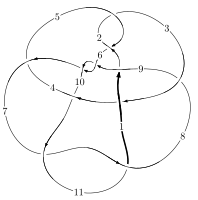
\includegraphics[width=112pt]{../../../GIT/diagram.site/Diagrams/png/538_11a_289.png}\\
\ \ \ A knot diagram\footnotemark}&
\allowdisplaybreaks
\textbf{Linearized knot diagam} \\
\cline{2-2}
 &
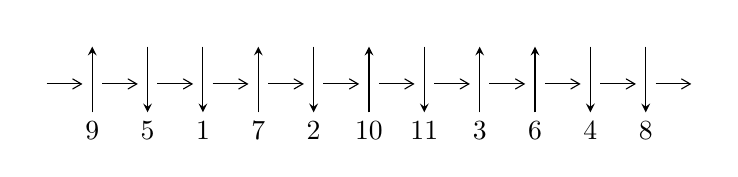
\begin{tikzpicture}[x=20pt, y=17pt]
	% nodes
	\node (C0) at (0, 0) {};
	\node (C1) at (1, 0) {};
	\node (C1U) at (1, +1) {};
	\node (C1D) at (1, -1) {9};

	\node (C2) at (2, 0) {};
	\node (C2U) at (2, +1) {};
	\node (C2D) at (2, -1) {5};

	\node (C3) at (3, 0) {};
	\node (C3U) at (3, +1) {};
	\node (C3D) at (3, -1) {1};

	\node (C4) at (4, 0) {};
	\node (C4U) at (4, +1) {};
	\node (C4D) at (4, -1) {7};

	\node (C5) at (5, 0) {};
	\node (C5U) at (5, +1) {};
	\node (C5D) at (5, -1) {2};

	\node (C6) at (6, 0) {};
	\node (C6U) at (6, +1) {};
	\node (C6D) at (6, -1) {10};

	\node (C7) at (7, 0) {};
	\node (C7U) at (7, +1) {};
	\node (C7D) at (7, -1) {11};

	\node (C8) at (8, 0) {};
	\node (C8U) at (8, +1) {};
	\node (C8D) at (8, -1) {3};

	\node (C9) at (9, 0) {};
	\node (C9U) at (9, +1) {};
	\node (C9D) at (9, -1) {6};

	\node (C10) at (10, 0) {};
	\node (C10U) at (10, +1) {};
	\node (C10D) at (10, -1) {4};

	\node (C11) at (11, 0) {};
	\node (C11U) at (11, +1) {};
	\node (C11D) at (11, -1) {8};
	\node (C12) at (12, 0) {};

	% arrows
	\draw[->,>={angle 60}]
	(C0) edge (C1) (C1) edge (C2) (C2) edge (C3) (C3) edge (C4) (C4) edge (C5) (C5) edge (C6) (C6) edge (C7) (C7) edge (C8) (C8) edge (C9) (C9) edge (C10) (C10) edge (C11) (C11) edge (C12) ;	\draw[->,>=stealth]
	(C1D) edge (C1U) (C2U) edge (C2D) (C3U) edge (C3D) (C4D) edge (C4U) (C5U) edge (C5D) (C6D) edge (C6U) (C7U) edge (C7D) (C8D) edge (C8U) (C9D) edge (C9U) (C10U) edge (C10D) (C11U) edge (C11D) ;
	\end{tikzpicture} \\
\hhline{~~} \\& 
\textbf{Solving Sequence} \\ \cline{2-2} 
 &
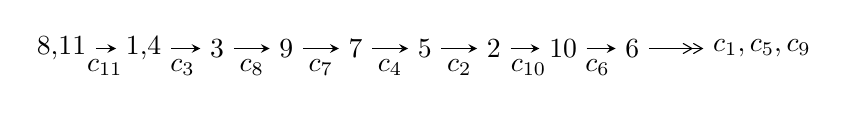
\begin{tikzpicture}[x=25pt, y=7pt]
	% node
	\node (A0) at (-1/8, 0) {8,11};
	\node (A1) at (17/16, 0) {1,4};
	\node (A2) at (17/8, 0) {3};
	\node (A3) at (25/8, 0) {9};
	\node (A4) at (33/8, 0) {7};
	\node (A5) at (41/8, 0) {5};
	\node (A6) at (49/8, 0) {2};
	\node (A7) at (57/8, 0) {10};
	\node (A8) at (65/8, 0) {6};
	\node (C1) at (1/2, -1) {$c_{11}$};
	\node (C2) at (13/8, -1) {$c_{3}$};
	\node (C3) at (21/8, -1) {$c_{8}$};
	\node (C4) at (29/8, -1) {$c_{7}$};
	\node (C5) at (37/8, -1) {$c_{4}$};
	\node (C6) at (45/8, -1) {$c_{2}$};
	\node (C7) at (53/8, -1) {$c_{10}$};
	\node (C8) at (61/8, -1) {$c_{6}$};
	\node (A9) at (10, 0) {$c_{1},c_{5},c_{9}$};

	% edge
	\draw[->,>=stealth]	
	(A0) edge (A1) (A1) edge (A2) (A2) edge (A3) (A3) edge (A4) (A4) edge (A5) (A5) edge (A6) (A6) edge (A7) (A7) edge (A8) ;
	\draw[->>,>={angle 60}]	
	(A8) edge (A9);
\end{tikzpicture} \\ 

\end{tabular} \\

\footnotetext{
The image of knot diagram is generated by the software ``\textbf{Draw programme}" developed by Andrew Bartholomew(\url{http://www.layer8.co.uk/maths/draw/index.htm\#Running-draw}), where we modified some parts for our purpose(\url{https://github.com/CATsTAILs/LinksPainter}).
}\phantom \\ \newline 
\centering \textbf{Ideals for irreducible components\footnotemark of $X_{\text{par}}$} 
 
\begin{align*}
I^u_{1}&=\langle 
-2.33884\times10^{224} u^{90}+2.00374\times10^{224} u^{89}+\cdots+1.85594\times10^{224} b-1.47160\times10^{225},\\
\phantom{I^u_{1}}&\phantom{= \langle  }-6.91616\times10^{224} u^{90}-7.19072\times10^{224} u^{89}+\cdots+1.85594\times10^{224} a+1.27904\times10^{226},\\
\phantom{I^u_{1}}&\phantom{= \langle  }u^{91}+u^{90}+\cdots-38 u-1\rangle \\
I^u_{2}&=\langle 
-21753030 u^{18}+6745274 u^{17}+\cdots+4200133 b-80944935,\\
\phantom{I^u_{2}}&\phantom{= \langle  }2155133 u^{18}-644977 u^{17}+\cdots+85717 a+7203604,\;u^{19}-7 u^{17}+\cdots+4 u+1\rangle \\
\\
\end{align*}
\raggedright * 2 irreducible components of $\dim_{\mathbb{C}}=0$, with total 110 representations.\\
\footnotetext{All coefficients of polynomials are rational numbers. But the coefficients are sometimes approximated in decimal forms when there is not enough margin.}
\newpage
\renewcommand{\arraystretch}{1}
\centering \section*{I. $I^u_{1}= \langle -2.34\times10^{224} u^{90}+2.00\times10^{224} u^{89}+\cdots+1.86\times10^{224} b-1.47\times10^{225},\;-6.92\times10^{224} u^{90}-7.19\times10^{224} u^{89}+\cdots+1.86\times10^{224} a+1.28\times10^{226},\;u^{91}+u^{90}+\cdots-38 u-1 \rangle$}
\flushleft \textbf{(i) Arc colorings}\\
\begin{tabular}{m{7pt} m{180pt} m{7pt} m{180pt} }
\flushright $a_{8}=$&$\begin{pmatrix}0\\u\end{pmatrix}$ \\
\flushright $a_{11}=$&$\begin{pmatrix}1\\0\end{pmatrix}$ \\
\flushright $a_{1}=$&$\begin{pmatrix}1\\u^2\end{pmatrix}$ \\
\flushright $a_{4}=$&$\begin{pmatrix}3.72650 u^{90}+3.87443 u^{89}+\cdots-1799.70 u-68.9163\\1.26019 u^{90}-1.07963 u^{89}+\cdots+176.719 u+7.92913\end{pmatrix}$ \\
\flushright $a_{3}=$&$\begin{pmatrix}4.76767 u^{90}+3.17976 u^{89}+\cdots-1632.33 u-61.1351\\3.22294 u^{90}-1.26978 u^{89}+\cdots+111.798 u+6.19329\end{pmatrix}$ \\
\flushright $a_{9}=$&$\begin{pmatrix}7.99747 u^{90}+1.78196 u^{89}+\cdots-1075.61 u-44.5830\\6.35087 u^{90}-0.377320 u^{89}+\cdots-261.022 u-6.24056\end{pmatrix}$ \\
\flushright $a_{7}=$&$\begin{pmatrix}u\\u\end{pmatrix}$ \\
\flushright $a_{5}=$&$\begin{pmatrix}6.40251 u^{90}+3.66084 u^{89}+\cdots-1896.70 u-71.4040\\3.93620 u^{90}-1.29323 u^{89}+\cdots+79.7178 u+5.44137\end{pmatrix}$ \\
\flushright $a_{2}=$&$\begin{pmatrix}-1.49138 u^{90}+0.843199 u^{89}+\cdots+578.943 u+31.1708\\-1.35638 u^{90}+0.0358487 u^{89}+\cdots+49.5120 u+0.205445\end{pmatrix}$ \\
\flushright $a_{10}=$&$\begin{pmatrix}5.66600 u^{90}-1.49334 u^{89}+\cdots+485.280 u+37.8985\\8.67471 u^{90}+0.525243 u^{89}+\cdots-589.369 u-19.3718\end{pmatrix}$ \\
\flushright $a_{6}=$&$\begin{pmatrix}-5.66191 u^{90}-2.29724 u^{89}+\cdots+1339.51 u+68.3501\\-2.09349 u^{90}+1.35317 u^{89}+\cdots-175.967 u-8.47779\end{pmatrix}$\\ \flushright $a_{6}=$&$\begin{pmatrix}-5.66191 u^{90}-2.29724 u^{89}+\cdots+1339.51 u+68.3501\\-2.09349 u^{90}+1.35317 u^{89}+\cdots-175.967 u-8.47779\end{pmatrix}$\\&\end{tabular}
\flushleft \textbf{(ii) Obstruction class $= -1$}\\~\\
\flushleft \textbf{(iii) Cusp Shapes $= -17.9996 u^{90}-14.8667 u^{89}+\cdots+4221.76 u+150.087$}\\~\\
\newpage\renewcommand{\arraystretch}{1}
\flushleft \textbf{(iv) u-Polynomials at the component}\newline \\
\begin{tabular}{m{50pt}|m{274pt}}
Crossings & \hspace{64pt}u-Polynomials at each crossing \\
\hline $$\begin{aligned}c_{1}\end{aligned}$$&$\begin{aligned}
&u^{91}-5 u^{90}+\cdots+244460 u-108400
\end{aligned}$\\
\hline $$\begin{aligned}c_{2},c_{5}\end{aligned}$$&$\begin{aligned}
&u^{91}+6 u^{90}+\cdots+757 u+1751
\end{aligned}$\\
\hline $$\begin{aligned}c_{3}\end{aligned}$$&$\begin{aligned}
&u^{91}-10 u^{90}+\cdots-36 u+1
\end{aligned}$\\
\hline $$\begin{aligned}c_{4}\end{aligned}$$&$\begin{aligned}
&u^{91}+9 u^{90}+\cdots+25 u+1
\end{aligned}$\\
\hline $$\begin{aligned}c_{6},c_{9}\end{aligned}$$&$\begin{aligned}
&u^{91}-2 u^{90}+\cdots-37 u+1117
\end{aligned}$\\
\hline $$\begin{aligned}c_{7},c_{11}\end{aligned}$$&$\begin{aligned}
&u^{91}+u^{90}+\cdots-38 u-1
\end{aligned}$\\
\hline $$\begin{aligned}c_{8}\end{aligned}$$&$\begin{aligned}
&u^{91}+u^{90}+\cdots+80 u+37
\end{aligned}$\\
\hline $$\begin{aligned}c_{10}\end{aligned}$$&$\begin{aligned}
&u^{91}+2 u^{90}+\cdots-46 u+4
\end{aligned}$\\
\hline
\end{tabular}\\~\\
\newpage\renewcommand{\arraystretch}{1}
\flushleft \textbf{(v) Riley Polynomials at the component}\newline \\
\begin{tabular}{m{50pt}|m{274pt}}
Crossings & \hspace{64pt}Riley Polynomials at each crossing \\
\hline $$\begin{aligned}c_{1}\end{aligned}$$&$\begin{aligned}
&y^{91}-37 y^{90}+\cdots+248464929200 y-11750560000
\end{aligned}$\\
\hline $$\begin{aligned}c_{2},c_{5}\end{aligned}$$&$\begin{aligned}
&y^{91}+58 y^{90}+\cdots-43405067 y-3066001
\end{aligned}$\\
\hline $$\begin{aligned}c_{3}\end{aligned}$$&$\begin{aligned}
&y^{91}-10 y^{90}+\cdots+128 y-1
\end{aligned}$\\
\hline $$\begin{aligned}c_{4}\end{aligned}$$&$\begin{aligned}
&y^{91}-3 y^{90}+\cdots+353 y-1
\end{aligned}$\\
\hline $$\begin{aligned}c_{6},c_{9}\end{aligned}$$&$\begin{aligned}
&y^{91}-74 y^{90}+\cdots-20772597 y-1247689
\end{aligned}$\\
\hline $$\begin{aligned}c_{7},c_{11}\end{aligned}$$&$\begin{aligned}
&y^{91}-65 y^{90}+\cdots+218 y-1
\end{aligned}$\\
\hline $$\begin{aligned}c_{8}\end{aligned}$$&$\begin{aligned}
&y^{91}+13 y^{90}+\cdots-186888 y-1369
\end{aligned}$\\
\hline $$\begin{aligned}c_{10}\end{aligned}$$&$\begin{aligned}
&y^{91}+48 y^{89}+\cdots-1780 y-16
\end{aligned}$\\
\hline
\end{tabular}\\~\\
\newpage\flushleft \textbf{(vi) Complex Volumes and Cusp Shapes}
$$\begin{array}{c|c|c}  
\text{Solutions to }I^u_{1}& \I (\text{vol} + \sqrt{-1}CS) & \text{Cusp shape}\\
 \hline 
\begin{aligned}
u &= \phantom{-}0.154514 + 1.000430 I \\
a &= \phantom{-}0.105188 + 0.509185 I \\
b &= \phantom{-}0.600669 - 0.721061 I\end{aligned}
 & \phantom{-}3.06412 + 2.24647 I & \phantom{-0.000000 } 0 \\ \hline\begin{aligned}
u &= \phantom{-}0.154514 - 1.000430 I \\
a &= \phantom{-}0.105188 - 0.509185 I \\
b &= \phantom{-}0.600669 + 0.721061 I\end{aligned}
 & \phantom{-}3.06412 - 2.24647 I & \phantom{-0.000000 } 0 \\ \hline\begin{aligned}
u &= -0.925483 + 0.337630 I \\
a &= \phantom{-}2.22116 + 0.06041 I \\
b &= -0.113347 - 0.257600 I\end{aligned}
 & \phantom{-}5.58118 + 7.27652 I & \phantom{-0.000000 } 0 \\ \hline\begin{aligned}
u &= -0.925483 - 0.337630 I \\
a &= \phantom{-}2.22116 - 0.06041 I \\
b &= -0.113347 + 0.257600 I\end{aligned}
 & \phantom{-}5.58118 - 7.27652 I & \phantom{-0.000000 } 0 \\ \hline\begin{aligned}
u &= \phantom{-}1.021280 + 0.097812 I \\
a &= \phantom{-}0.013238 + 0.538865 I \\
b &= \phantom{-}0.028178 - 1.308020 I\end{aligned}
 & \phantom{-}4.96637 + 0.14906 I & \phantom{-0.000000 } 0 \\ \hline\begin{aligned}
u &= \phantom{-}1.021280 - 0.097812 I \\
a &= \phantom{-}0.013238 - 0.538865 I \\
b &= \phantom{-}0.028178 + 1.308020 I\end{aligned}
 & \phantom{-}4.96637 - 0.14906 I & \phantom{-0.000000 } 0 \\ \hline\begin{aligned}
u &= \phantom{-}0.242468 + 1.000660 I \\
a &= \phantom{-}0.286579 - 0.228220 I \\
b &= -0.338311 + 0.628821 I\end{aligned}
 & \phantom{-}1.90649 + 1.11668 I & \phantom{-0.000000 } 0 \\ \hline\begin{aligned}
u &= \phantom{-}0.242468 - 1.000660 I \\
a &= \phantom{-}0.286579 + 0.228220 I \\
b &= -0.338311 - 0.628821 I\end{aligned}
 & \phantom{-}1.90649 - 1.11668 I & \phantom{-0.000000 } 0 \\ \hline\begin{aligned}
u &= \phantom{-}0.177856 + 0.940264 I \\
a &= -0.0109358 - 0.0657220 I \\
b &= \phantom{-}0.615843 + 1.111660 I\end{aligned}
 & \phantom{-}4.35772 - 5.92655 I & \phantom{-0.000000 } 0 \\ \hline\begin{aligned}
u &= \phantom{-}0.177856 - 0.940264 I \\
a &= -0.0109358 + 0.0657220 I \\
b &= \phantom{-}0.615843 - 1.111660 I\end{aligned}
 & \phantom{-}4.35772 + 5.92655 I & \phantom{-0.000000 } 0\\
 \hline 
 \end{array}$$\newpage$$\begin{array}{c|c|c}  
\text{Solutions to }I^u_{1}& \I (\text{vol} + \sqrt{-1}CS) & \text{Cusp shape}\\
 \hline 
\begin{aligned}
u &= \phantom{-}0.853700 + 0.606656 I \\
a &= \phantom{-}0.672847 + 0.305259 I \\
b &= -0.160836 + 0.461008 I\end{aligned}
 & \phantom{-}2.01129 + 0.63862 I & \phantom{-0.000000 } 0 \\ \hline\begin{aligned}
u &= \phantom{-}0.853700 - 0.606656 I \\
a &= \phantom{-}0.672847 - 0.305259 I \\
b &= -0.160836 - 0.461008 I\end{aligned}
 & \phantom{-}2.01129 - 0.63862 I & \phantom{-0.000000 } 0 \\ \hline\begin{aligned}
u &= -0.254816 + 0.881587 I \\
a &= \phantom{-}0.137178 - 0.146852 I \\
b &= \phantom{-}0.310437 - 0.630125 I\end{aligned}
 & \phantom{-}0.01106 + 2.05657 I & \phantom{-0.000000 } 0 \\ \hline\begin{aligned}
u &= -0.254816 - 0.881587 I \\
a &= \phantom{-}0.137178 + 0.146852 I \\
b &= \phantom{-}0.310437 + 0.630125 I\end{aligned}
 & \phantom{-}0.01106 - 2.05657 I & \phantom{-0.000000 } 0 \\ \hline\begin{aligned}
u &= -0.638896 + 0.646429 I \\
a &= -0.178496 + 1.303700 I \\
b &= \phantom{-}0.198949 - 0.951481 I\end{aligned}
 & \phantom{-}6.40508 - 3.26778 I & \phantom{-0.000000 } 0 \\ \hline\begin{aligned}
u &= -0.638896 - 0.646429 I \\
a &= -0.178496 - 1.303700 I \\
b &= \phantom{-}0.198949 + 0.951481 I\end{aligned}
 & \phantom{-}6.40508 + 3.26778 I & \phantom{-0.000000 } 0 \\ \hline\begin{aligned}
u &= \phantom{-}0.445566 + 0.776682 I \\
a &= -0.420019 - 0.743253 I \\
b &= \phantom{-}0.648716 - 1.061710 I\end{aligned}
 & \phantom{-}8.11082 + 3.81719 I & \phantom{-0.000000 } 0 \\ \hline\begin{aligned}
u &= \phantom{-}0.445566 - 0.776682 I \\
a &= -0.420019 + 0.743253 I \\
b &= \phantom{-}0.648716 + 1.061710 I\end{aligned}
 & \phantom{-}8.11082 - 3.81719 I & \phantom{-0.000000 } 0 \\ \hline\begin{aligned}
u &= -1.102810 + 0.120356 I \\
a &= \phantom{-}1.112970 + 0.716630 I \\
b &= \phantom{-}1.03514 + 1.52926 I\end{aligned}
 & -0.86513 + 3.43410 I & \phantom{-0.000000 } 0 \\ \hline\begin{aligned}
u &= -1.102810 - 0.120356 I \\
a &= \phantom{-}1.112970 - 0.716630 I \\
b &= \phantom{-}1.03514 - 1.52926 I\end{aligned}
 & -0.86513 - 3.43410 I & \phantom{-0.000000 } 0\\
 \hline 
 \end{array}$$\newpage$$\begin{array}{c|c|c}  
\text{Solutions to }I^u_{1}& \I (\text{vol} + \sqrt{-1}CS) & \text{Cusp shape}\\
 \hline 
\begin{aligned}
u &= \phantom{-}1.036080 + 0.399219 I \\
a &= -1.86514 - 0.23806 I \\
b &= -1.39914 - 1.31114 I\end{aligned}
 & \phantom{-}6.27718 - 8.20883 I & \phantom{-0.000000 } 0 \\ \hline\begin{aligned}
u &= \phantom{-}1.036080 - 0.399219 I \\
a &= -1.86514 + 0.23806 I \\
b &= -1.39914 + 1.31114 I\end{aligned}
 & \phantom{-}6.27718 + 8.20883 I & \phantom{-0.000000 } 0 \\ \hline\begin{aligned}
u &= -1.122850 + 0.028210 I \\
a &= -1.87730 + 0.53457 I \\
b &= -1.36440 + 1.26320 I\end{aligned}
 & -3.52236 + 1.23004 I & \phantom{-0.000000 } 0 \\ \hline\begin{aligned}
u &= -1.122850 - 0.028210 I \\
a &= -1.87730 - 0.53457 I \\
b &= -1.36440 - 1.26320 I\end{aligned}
 & -3.52236 - 1.23004 I & \phantom{-0.000000 } 0 \\ \hline\begin{aligned}
u &= \phantom{-}1.088340 + 0.354136 I \\
a &= \phantom{-}1.88933 - 0.00662 I \\
b &= \phantom{-}0.689405 + 0.508116 I\end{aligned}
 & \phantom{-}1.41670 - 5.22000 I & \phantom{-0.000000 } 0 \\ \hline\begin{aligned}
u &= \phantom{-}1.088340 - 0.354136 I \\
a &= \phantom{-}1.88933 + 0.00662 I \\
b &= \phantom{-}0.689405 - 0.508116 I\end{aligned}
 & \phantom{-}1.41670 + 5.22000 I & \phantom{-0.000000 } 0 \\ \hline\begin{aligned}
u &= \phantom{-}0.107319 + 1.155390 I \\
a &= -0.0450787 + 0.0302813 I \\
b &= -0.666347 - 1.032170 I\end{aligned}
 & \phantom{-}8.3586 - 11.6518 I & \phantom{-0.000000 } 0 \\ \hline\begin{aligned}
u &= \phantom{-}0.107319 - 1.155390 I \\
a &= -0.0450787 - 0.0302813 I \\
b &= -0.666347 + 1.032170 I\end{aligned}
 & \phantom{-}8.3586 + 11.6518 I & \phantom{-0.000000 } 0 \\ \hline\begin{aligned}
u &= -1.160610 + 0.125188 I \\
a &= \phantom{-}2.07171 + 0.76197 I \\
b &= \phantom{-}0.835112 - 0.755768 I\end{aligned}
 & \phantom{-}2.65519 + 7.24321 I & \phantom{-0.000000 } 0 \\ \hline\begin{aligned}
u &= -1.160610 - 0.125188 I \\
a &= \phantom{-}2.07171 - 0.76197 I \\
b &= \phantom{-}0.835112 + 0.755768 I\end{aligned}
 & \phantom{-}2.65519 - 7.24321 I & \phantom{-0.000000 } 0\\
 \hline 
 \end{array}$$\newpage$$\begin{array}{c|c|c}  
\text{Solutions to }I^u_{1}& \I (\text{vol} + \sqrt{-1}CS) & \text{Cusp shape}\\
 \hline 
\begin{aligned}
u &= -1.18021\phantom{ +0.000000I} \\
a &= -2.85483\phantom{ +0.000000I} \\
b &= -1.34979\phantom{ +0.000000I}\end{aligned}
 & -2.49691\phantom{ +0.000000I} & \phantom{-0.000000 } 0 \\ \hline\begin{aligned}
u &= \phantom{-}1.186300 + 0.048699 I \\
a &= -1.59766 - 0.40123 I \\
b &= -0.878174 + 0.318552 I\end{aligned}
 & -4.89749 - 1.53348 I & \phantom{-0.000000 } 0 \\ \hline\begin{aligned}
u &= \phantom{-}1.186300 - 0.048699 I \\
a &= -1.59766 + 0.40123 I \\
b &= -0.878174 - 0.318552 I\end{aligned}
 & -4.89749 + 1.53348 I & \phantom{-0.000000 } 0 \\ \hline\begin{aligned}
u &= -1.182020 + 0.116137 I \\
a &= \phantom{-}1.273900 - 0.281879 I \\
b &= \phantom{-}1.120750 - 0.771869 I\end{aligned}
 & -2.65839 + 0.87469 I & \phantom{-0.000000 } 0 \\ \hline\begin{aligned}
u &= -1.182020 - 0.116137 I \\
a &= \phantom{-}1.273900 + 0.281879 I \\
b &= \phantom{-}1.120750 + 0.771869 I\end{aligned}
 & -2.65839 - 0.87469 I & \phantom{-0.000000 } 0 \\ \hline\begin{aligned}
u &= \phantom{-}1.180210 + 0.162238 I \\
a &= \phantom{-}1.040030 - 0.496367 I \\
b &= \phantom{-}0.644086 + 0.744559 I\end{aligned}
 & -2.79141 - 4.21603 I & \phantom{-0.000000 } 0 \\ \hline\begin{aligned}
u &= \phantom{-}1.180210 - 0.162238 I \\
a &= \phantom{-}1.040030 + 0.496367 I \\
b &= \phantom{-}0.644086 - 0.744559 I\end{aligned}
 & -2.79141 + 4.21603 I & \phantom{-0.000000 } 0 \\ \hline\begin{aligned}
u &= -0.652969 + 0.474285 I \\
a &= -1.09565 - 1.00396 I \\
b &= -0.972670 + 0.215028 I\end{aligned}
 & \phantom{-}1.29512 + 2.45316 I & \phantom{-0.000000 } 0 \\ \hline\begin{aligned}
u &= -0.652969 - 0.474285 I \\
a &= -1.09565 + 1.00396 I \\
b &= -0.972670 - 0.215028 I\end{aligned}
 & \phantom{-}1.29512 - 2.45316 I & \phantom{-0.000000 } 0 \\ \hline\begin{aligned}
u &= \phantom{-}1.189900 + 0.165844 I \\
a &= \phantom{-}1.98196 - 0.66468 I \\
b &= \phantom{-}2.04084 - 0.86369 I\end{aligned}
 & \phantom{-}2.09247 - 7.92588 I & \phantom{-0.000000 } 0\\
 \hline 
 \end{array}$$\newpage$$\begin{array}{c|c|c}  
\text{Solutions to }I^u_{1}& \I (\text{vol} + \sqrt{-1}CS) & \text{Cusp shape}\\
 \hline 
\begin{aligned}
u &= \phantom{-}1.189900 - 0.165844 I \\
a &= \phantom{-}1.98196 + 0.66468 I \\
b &= \phantom{-}2.04084 + 0.86369 I\end{aligned}
 & \phantom{-}2.09247 + 7.92588 I & \phantom{-0.000000 } 0 \\ \hline\begin{aligned}
u &= -1.157580 + 0.336921 I \\
a &= -0.556616 - 0.531666 I \\
b &= -0.493201 - 0.788878 I\end{aligned}
 & -1.22092 + 2.30068 I & \phantom{-0.000000 } 0 \\ \hline\begin{aligned}
u &= -1.157580 - 0.336921 I \\
a &= -0.556616 + 0.531666 I \\
b &= -0.493201 + 0.788878 I\end{aligned}
 & -1.22092 - 2.30068 I & \phantom{-0.000000 } 0 \\ \hline\begin{aligned}
u &= \phantom{-}1.21568\phantom{ +0.000000I} \\
a &= -2.64009\phantom{ +0.000000I} \\
b &= -2.59413\phantom{ +0.000000I}\end{aligned}
 & -3.13944\phantom{ +0.000000I} & \phantom{-0.000000 } 0 \\ \hline\begin{aligned}
u &= \phantom{-}0.384760 + 0.675310 I \\
a &= -0.278767 - 0.486904 I \\
b &= -0.344151 + 0.878398 I\end{aligned}
 & \phantom{-}3.59264 + 1.28182 I & \phantom{-}5.23084 + 0. I\phantom{ +0.000000I} \\ \hline\begin{aligned}
u &= \phantom{-}0.384760 - 0.675310 I \\
a &= -0.278767 + 0.486904 I \\
b &= -0.344151 - 0.878398 I\end{aligned}
 & \phantom{-}3.59264 - 1.28182 I & \phantom{-}5.23084 + 0. I\phantom{ +0.000000I} \\ \hline\begin{aligned}
u &= \phantom{-}0.742449 + 0.188337 I \\
a &= -1.55951 - 1.79492 I \\
b &= -0.000176 - 0.473465 I\end{aligned}
 & \phantom{-}5.66154 - 1.41791 I & \phantom{-}1.45782 + 3.29961 I \\ \hline\begin{aligned}
u &= \phantom{-}0.742449 - 0.188337 I \\
a &= -1.55951 + 1.79492 I \\
b &= -0.000176 + 0.473465 I\end{aligned}
 & \phantom{-}5.66154 + 1.41791 I & \phantom{-}1.45782 - 3.29961 I \\ \hline\begin{aligned}
u &= -1.206280 + 0.364725 I \\
a &= \phantom{-}2.03871 - 0.29594 I \\
b &= \phantom{-}1.30237 - 1.17332 I\end{aligned}
 & \phantom{-}5.59028 + 4.35769 I & \phantom{-0.000000 } 0 \\ \hline\begin{aligned}
u &= -1.206280 - 0.364725 I \\
a &= \phantom{-}2.03871 + 0.29594 I \\
b &= \phantom{-}1.30237 + 1.17332 I\end{aligned}
 & \phantom{-}5.59028 - 4.35769 I & \phantom{-0.000000 } 0\\
 \hline 
 \end{array}$$\newpage$$\begin{array}{c|c|c}  
\text{Solutions to }I^u_{1}& \I (\text{vol} + \sqrt{-1}CS) & \text{Cusp shape}\\
 \hline 
\begin{aligned}
u &= -0.111033 + 0.728216 I \\
a &= \phantom{-}0.126141 - 0.073845 I \\
b &= -0.716226 - 1.210120 I\end{aligned}
 & \phantom{-}8.95711 - 0.33313 I & \phantom{-}8.32553 + 0.37349 I \\ \hline\begin{aligned}
u &= -0.111033 - 0.728216 I \\
a &= \phantom{-}0.126141 + 0.073845 I \\
b &= -0.716226 + 1.210120 I\end{aligned}
 & \phantom{-}8.95711 + 0.33313 I & \phantom{-}8.32553 - 0.37349 I \\ \hline\begin{aligned}
u &= -0.108439 + 0.723146 I \\
a &= \phantom{-}1.007320 - 0.414367 I \\
b &= -0.285144 + 0.976899 I\end{aligned}
 & \phantom{-}3.40759 + 0.78642 I & \phantom{-}2.69705 - 0.95790 I \\ \hline\begin{aligned}
u &= -0.108439 - 0.723146 I \\
a &= \phantom{-}1.007320 + 0.414367 I \\
b &= -0.285144 - 0.976899 I\end{aligned}
 & \phantom{-}3.40759 - 0.78642 I & \phantom{-}2.69705 + 0.95790 I \\ \hline\begin{aligned}
u &= -1.252140 + 0.238107 I \\
a &= -0.889184 + 0.812716 I \\
b &= -0.0532821 + 0.1257370 I\end{aligned}
 & -0.24585 + 2.81188 I & \phantom{-0.000000 } 0 \\ \hline\begin{aligned}
u &= -1.252140 - 0.238107 I \\
a &= -0.889184 - 0.812716 I \\
b &= -0.0532821 - 0.1257370 I\end{aligned}
 & -0.24585 - 2.81188 I & \phantom{-0.000000 } 0 \\ \hline\begin{aligned}
u &= -0.076027 + 1.282950 I \\
a &= \phantom{-}0.011447 + 0.142790 I \\
b &= -0.464789 + 0.521507 I\end{aligned}
 & \phantom{-}2.33628 + 5.25645 I & \phantom{-0.000000 } 0 \\ \hline\begin{aligned}
u &= -0.076027 - 1.282950 I \\
a &= \phantom{-}0.011447 - 0.142790 I \\
b &= -0.464789 - 0.521507 I\end{aligned}
 & \phantom{-}2.33628 - 5.25645 I & \phantom{-0.000000 } 0 \\ \hline\begin{aligned}
u &= \phantom{-}1.275300 + 0.163827 I \\
a &= \phantom{-}0.688235 + 1.032460 I \\
b &= \phantom{-}0.55547 + 1.93773 I\end{aligned}
 & -1.17722 - 3.75603 I & \phantom{-0.000000 } 0 \\ \hline\begin{aligned}
u &= \phantom{-}1.275300 - 0.163827 I \\
a &= \phantom{-}0.688235 - 1.032460 I \\
b &= \phantom{-}0.55547 - 1.93773 I\end{aligned}
 & -1.17722 + 3.75603 I & \phantom{-0.000000 } 0\\
 \hline 
 \end{array}$$\newpage$$\begin{array}{c|c|c}  
\text{Solutions to }I^u_{1}& \I (\text{vol} + \sqrt{-1}CS) & \text{Cusp shape}\\
 \hline 
\begin{aligned}
u &= \phantom{-}1.307530 + 0.476334 I \\
a &= \phantom{-}1.246040 - 0.069703 I \\
b &= \phantom{-}0.898713 + 1.080480 I\end{aligned}
 & -1.76672 - 6.33798 I & \phantom{-0.000000 } 0 \\ \hline\begin{aligned}
u &= \phantom{-}1.307530 - 0.476334 I \\
a &= \phantom{-}1.246040 + 0.069703 I \\
b &= \phantom{-}0.898713 - 1.080480 I\end{aligned}
 & -1.76672 + 6.33798 I & \phantom{-0.000000 } 0 \\ \hline\begin{aligned}
u &= \phantom{-}1.31886 + 0.56606 I \\
a &= -1.308320 + 0.259548 I \\
b &= -0.787261 - 1.024100 I\end{aligned}
 & -0.57560 - 7.98468 I & \phantom{-0.000000 } 0 \\ \hline\begin{aligned}
u &= \phantom{-}1.31886 - 0.56606 I \\
a &= -1.308320 - 0.259548 I \\
b &= -0.787261 + 1.024100 I\end{aligned}
 & -0.57560 + 7.98468 I & \phantom{-0.000000 } 0 \\ \hline\begin{aligned}
u &= \phantom{-}1.37950 + 0.43905 I \\
a &= -1.370230 - 0.119084 I \\
b &= -1.078280 - 0.817964 I\end{aligned}
 & -4.95903 - 6.92588 I & \phantom{-0.000000 } 0 \\ \hline\begin{aligned}
u &= \phantom{-}1.37950 - 0.43905 I \\
a &= -1.370230 + 0.119084 I \\
b &= -1.078280 + 0.817964 I\end{aligned}
 & -4.95903 + 6.92588 I & \phantom{-0.000000 } 0 \\ \hline\begin{aligned}
u &= -1.38281 + 0.43401 I \\
a &= -1.61543 + 0.36310 I \\
b &= -1.15059 + 1.32568 I\end{aligned}
 & -0.50912 + 10.85460 I & \phantom{-0.000000 } 0 \\ \hline\begin{aligned}
u &= -1.38281 - 0.43401 I \\
a &= -1.61543 - 0.36310 I \\
b &= -1.15059 - 1.32568 I\end{aligned}
 & -0.50912 - 10.85460 I & \phantom{-0.000000 } 0 \\ \hline\begin{aligned}
u &= -1.42369 + 0.35800 I \\
a &= \phantom{-}0.945721 - 0.055490 I \\
b &= \phantom{-}0.859159 - 0.722591 I\end{aligned}
 & -3.55361 + 0.99335 I & \phantom{-0.000000 } 0 \\ \hline\begin{aligned}
u &= -1.42369 - 0.35800 I \\
a &= \phantom{-}0.945721 + 0.055490 I \\
b &= \phantom{-}0.859159 + 0.722591 I\end{aligned}
 & -3.55361 - 0.99335 I & \phantom{-0.000000 } 0\\
 \hline 
 \end{array}$$\newpage$$\begin{array}{c|c|c}  
\text{Solutions to }I^u_{1}& \I (\text{vol} + \sqrt{-1}CS) & \text{Cusp shape}\\
 \hline 
\begin{aligned}
u &= -1.36659 + 0.56938 I \\
a &= -0.664984 - 0.131205 I \\
b &= -0.556829 - 0.042970 I\end{aligned}
 & -1.16547 + 2.61720 I & \phantom{-0.000000 } 0 \\ \hline\begin{aligned}
u &= -1.36659 - 0.56938 I \\
a &= -0.664984 + 0.131205 I \\
b &= -0.556829 + 0.042970 I\end{aligned}
 & -1.16547 - 2.61720 I & \phantom{-0.000000 } 0 \\ \hline\begin{aligned}
u &= -1.29894 + 0.73144 I \\
a &= \phantom{-}0.745343 + 0.279706 I \\
b &= \phantom{-}0.921207 - 0.133086 I\end{aligned}
 & -0.26793 + 3.39964 I & \phantom{-0.000000 } 0 \\ \hline\begin{aligned}
u &= -1.29894 - 0.73144 I \\
a &= \phantom{-}0.745343 - 0.279706 I \\
b &= \phantom{-}0.921207 + 0.133086 I\end{aligned}
 & -0.26793 - 3.39964 I & \phantom{-0.000000 } 0 \\ \hline\begin{aligned}
u &= -1.40518 + 0.52888 I \\
a &= \phantom{-}1.50498 - 0.17996 I \\
b &= \phantom{-}1.09047 - 1.26911 I\end{aligned}
 & \phantom{-}3.6407 + 17.5515 I & \phantom{-0.000000 } 0 \\ \hline\begin{aligned}
u &= -1.40518 - 0.52888 I \\
a &= \phantom{-}1.50498 + 0.17996 I \\
b &= \phantom{-}1.09047 + 1.26911 I\end{aligned}
 & \phantom{-}3.6407 - 17.5515 I & \phantom{-0.000000 } 0 \\ \hline\begin{aligned}
u &= \phantom{-}1.40186 + 0.55296 I \\
a &= \phantom{-}1.263570 + 0.016688 I \\
b &= \phantom{-}1.12314 + 0.88528 I\end{aligned}
 & -2.28030 - 11.49490 I & \phantom{-0.000000 } 0 \\ \hline\begin{aligned}
u &= \phantom{-}1.40186 - 0.55296 I \\
a &= \phantom{-}1.263570 - 0.016688 I \\
b &= \phantom{-}1.12314 - 0.88528 I\end{aligned}
 & -2.28030 + 11.49490 I & \phantom{-0.000000 } 0 \\ \hline\begin{aligned}
u &= \phantom{-}1.53245 + 0.10660 I \\
a &= \phantom{-}0.161918 - 0.793466 I \\
b &= \phantom{-}0.293938 - 0.826547 I\end{aligned}
 & \phantom{-}3.82025 - 2.68111 I & \phantom{-0.000000 } 0 \\ \hline\begin{aligned}
u &= \phantom{-}1.53245 - 0.10660 I \\
a &= \phantom{-}0.161918 + 0.793466 I \\
b &= \phantom{-}0.293938 + 0.826547 I\end{aligned}
 & \phantom{-}3.82025 + 2.68111 I & \phantom{-0.000000 } 0\\
 \hline 
 \end{array}$$\newpage$$\begin{array}{c|c|c}  
\text{Solutions to }I^u_{1}& \I (\text{vol} + \sqrt{-1}CS) & \text{Cusp shape}\\
 \hline 
\begin{aligned}
u &= -1.44221 + 0.56336 I \\
a &= -0.816698 - 0.016295 I \\
b &= -0.598691 + 0.733628 I\end{aligned}
 & -3.54164 + 5.12239 I & \phantom{-0.000000 } 0 \\ \hline\begin{aligned}
u &= -1.44221 - 0.56336 I \\
a &= -0.816698 + 0.016295 I \\
b &= -0.598691 - 0.733628 I\end{aligned}
 & -3.54164 - 5.12239 I & \phantom{-0.000000 } 0 \\ \hline\begin{aligned}
u &= -0.368779 + 0.110817 I \\
a &= -1.79536 - 2.58891 I \\
b &= -0.816998 - 0.117532 I\end{aligned}
 & \phantom{-}1.19636 + 2.45261 I & -0.717024 - 0.766803 I \\ \hline\begin{aligned}
u &= -0.368779 - 0.110817 I \\
a &= -1.79536 + 2.58891 I \\
b &= -0.816998 + 0.117532 I\end{aligned}
 & \phantom{-}1.19636 - 2.45261 I & -0.717024 + 0.766803 I \\ \hline\begin{aligned}
u &= \phantom{-}1.38721 + 1.01014 I \\
a &= -0.186583 - 0.220285 I \\
b &= \phantom{-}0.172084 - 0.445375 I\end{aligned}
 & \phantom{-}4.73531 + 4.60663 I & \phantom{-0.000000 } 0 \\ \hline\begin{aligned}
u &= \phantom{-}1.38721 - 1.01014 I \\
a &= -0.186583 + 0.220285 I \\
b &= \phantom{-}0.172084 + 0.445375 I\end{aligned}
 & \phantom{-}4.73531 - 4.60663 I & \phantom{-0.000000 } 0 \\ \hline\begin{aligned}
u &= -0.178246 + 0.041738 I \\
a &= \phantom{-}1.23300 - 3.24629 I \\
b &= \phantom{-}0.634063 - 0.439863 I\end{aligned}
 & -1.14670 + 1.01760 I & -7.01569 - 3.15061 I \\ \hline\begin{aligned}
u &= -0.178246 - 0.041738 I \\
a &= \phantom{-}1.23300 + 3.24629 I \\
b &= \phantom{-}0.634063 + 0.439863 I\end{aligned}
 & -1.14670 - 1.01760 I & -7.01569 + 3.15061 I \\ \hline\begin{aligned}
u &= -0.0746543 + 0.0952110 I \\
a &= \phantom{-}1.77275 + 9.76874 I \\
b &= -1.077510 + 0.073135 I\end{aligned}
 & \phantom{-}5.66062 + 6.42858 I & \phantom{-}4.18077 - 5.08743 I \\ \hline\begin{aligned}
u &= -0.0746543 - 0.0952110 I \\
a &= \phantom{-}1.77275 - 9.76874 I \\
b &= -1.077510 - 0.073135 I\end{aligned}
 & \phantom{-}5.66062 - 6.42858 I & \phantom{-}4.18077 + 5.08743 I\\
 \hline 
 \end{array}$$\newpage$$\begin{array}{c|c|c}  
\text{Solutions to }I^u_{1}& \I (\text{vol} + \sqrt{-1}CS) & \text{Cusp shape}\\
 \hline 
\begin{aligned}
u &= -0.0762905\phantom{ +0.000000I} \\
a &= -9.34370\phantom{ +0.000000I} \\
b &= \phantom{-}1.33912\phantom{ +0.000000I}\end{aligned}
 & \phantom{-}0.594707\phantom{ +0.000000I} & \phantom{-}14.6100\phantom{ +0.000000I}\\
 \hline 
 \end{array}$$\newpage\newpage\renewcommand{\arraystretch}{1}
\centering \section*{II. $I^u_{2}= \langle -2.18\times10^{7} u^{18}+6.75\times10^{6} u^{17}+\cdots+4.20\times10^{6} b-8.09\times10^{7},\;2.16\times10^{6} u^{18}-6.45\times10^{5} u^{17}+\cdots+8.57\times10^{4} a+7.20\times10^{6},\;u^{19}-7 u^{17}+\cdots+4 u+1 \rangle$}
\flushleft \textbf{(i) Arc colorings}\\
\begin{tabular}{m{7pt} m{180pt} m{7pt} m{180pt} }
\flushright $a_{8}=$&$\begin{pmatrix}0\\u\end{pmatrix}$ \\
\flushright $a_{11}=$&$\begin{pmatrix}1\\0\end{pmatrix}$ \\
\flushright $a_{1}=$&$\begin{pmatrix}1\\u^2\end{pmatrix}$ \\
\flushright $a_{4}=$&$\begin{pmatrix}-25.1424 u^{18}+7.52449 u^{17}+\cdots-55.3865 u-84.0394\\5.17913 u^{18}-1.60597 u^{17}+\cdots+15.0703 u+19.2720\end{pmatrix}$ \\
\flushright $a_{3}=$&$\begin{pmatrix}-17.0714 u^{18}+5.18151 u^{17}+\cdots-35.3606 u-57.2429\\6.31136 u^{18}-1.60760 u^{17}+\cdots+16.3713 u+21.6150\end{pmatrix}$ \\
\flushright $a_{9}=$&$\begin{pmatrix}-13.3715 u^{18}+4.54857 u^{17}+\cdots-35.2371 u-43.3166\\1.94298 u^{18}-0.557214 u^{17}+\cdots+8.03710 u+6.25202\end{pmatrix}$ \\
\flushright $a_{7}=$&$\begin{pmatrix}u\\u\end{pmatrix}$ \\
\flushright $a_{5}=$&$\begin{pmatrix}-22.4896 u^{18}+6.87259 u^{17}+\cdots-49.1862 u-74.9089\\7.83195 u^{18}-2.25787 u^{17}+\cdots+21.2706 u+28.4025\end{pmatrix}$ \\
\flushright $a_{2}=$&$\begin{pmatrix}-26.8720 u^{18}+8.45143 u^{17}+\cdots-65.5699 u-88.5854\\8.06329 u^{18}-2.48624 u^{17}+\cdots+20.4130 u+24.7635\end{pmatrix}$ \\
\flushright $a_{10}=$&$\begin{pmatrix}3.55883 u^{18}-1.36223 u^{17}+\cdots+19.7553 u+11.9319\\1.28891 u^{18}-0.0106904 u^{17}+\cdots-1.10453 u+5.13136\end{pmatrix}$ \\
\flushright $a_{6}=$&$\begin{pmatrix}-9.79070 u^{18}+3.22584 u^{17}+\cdots-31.9356 u-28.8417\\-1.34165 u^{18}+0.268330 u^{17}+\cdots+3.99462 u-3.76913\end{pmatrix}$\\ \flushright $a_{6}=$&$\begin{pmatrix}-9.79070 u^{18}+3.22584 u^{17}+\cdots-31.9356 u-28.8417\\-1.34165 u^{18}+0.268330 u^{17}+\cdots+3.99462 u-3.76913\end{pmatrix}$\\&\end{tabular}
\flushleft \textbf{(ii) Obstruction class $= 1$}\\~\\
\flushleft \textbf{(iii) Cusp Shapes $= -\frac{15291933}{4200133} u^{18}+\frac{12321059}{4200133} u^{17}+\cdots-\frac{152094849}{4200133} u-\frac{21932593}{4200133}$}\\~\\
\newpage\renewcommand{\arraystretch}{1}
\flushleft \textbf{(iv) u-Polynomials at the component}\newline \\
\begin{tabular}{m{50pt}|m{274pt}}
Crossings & \hspace{64pt}u-Polynomials at each crossing \\
\hline $$\begin{aligned}c_{1}\end{aligned}$$&$\begin{aligned}
&u^{19}- u^{17}+\cdots-6 u+1
\end{aligned}$\\
\hline $$\begin{aligned}c_{2}\end{aligned}$$&$\begin{aligned}
&u^{19}-7 u^{18}+\cdots+3 u-1
\end{aligned}$\\
\hline $$\begin{aligned}c_{3}\end{aligned}$$&$\begin{aligned}
&u^{19}+3 u^{18}+\cdots+2 u+1
\end{aligned}$\\
\hline $$\begin{aligned}c_{4}\end{aligned}$$&$\begin{aligned}
&u^{19}+2 u^{18}+\cdots+u-1
\end{aligned}$\\
\hline $$\begin{aligned}c_{5}\end{aligned}$$&$\begin{aligned}
&u^{19}+7 u^{18}+\cdots+3 u+1
\end{aligned}$\\
\hline $$\begin{aligned}c_{6}\end{aligned}$$&$\begin{aligned}
&u^{19}- u^{18}+\cdots+5 u+1
\end{aligned}$\\
\hline $$\begin{aligned}c_{7}\end{aligned}$$&$\begin{aligned}
&u^{19}-7 u^{17}+\cdots+4 u-1
\end{aligned}$\\
\hline $$\begin{aligned}c_{8}\end{aligned}$$&$\begin{aligned}
&u^{19}+2 u^{17}+\cdots-4 u-1
\end{aligned}$\\
\hline $$\begin{aligned}c_{9}\end{aligned}$$&$\begin{aligned}
&u^{19}+u^{18}+\cdots+5 u-1
\end{aligned}$\\
\hline $$\begin{aligned}c_{10}\end{aligned}$$&$\begin{aligned}
&u^{19}+u^{18}+\cdots-3 u-1
\end{aligned}$\\
\hline $$\begin{aligned}c_{11}\end{aligned}$$&$\begin{aligned}
&u^{19}-7 u^{17}+\cdots+4 u+1
\end{aligned}$\\
\hline
\end{tabular}\\~\\
\newpage\renewcommand{\arraystretch}{1}
\flushleft \textbf{(v) Riley Polynomials at the component}\newline \\
\begin{tabular}{m{50pt}|m{274pt}}
Crossings & \hspace{64pt}Riley Polynomials at each crossing \\
\hline $$\begin{aligned}c_{1}\end{aligned}$$&$\begin{aligned}
&y^{19}-2 y^{18}+\cdots+46 y-1
\end{aligned}$\\
\hline $$\begin{aligned}c_{2},c_{5}\end{aligned}$$&$\begin{aligned}
&y^{19}+9 y^{18}+\cdots-15 y-1
\end{aligned}$\\
\hline $$\begin{aligned}c_{3}\end{aligned}$$&$\begin{aligned}
&y^{19}-11 y^{18}+\cdots-4 y-1
\end{aligned}$\\
\hline $$\begin{aligned}c_{4}\end{aligned}$$&$\begin{aligned}
&y^{19}-4 y^{18}+\cdots+13 y-1
\end{aligned}$\\
\hline $$\begin{aligned}c_{6},c_{9}\end{aligned}$$&$\begin{aligned}
&y^{19}-15 y^{18}+\cdots+31 y-1
\end{aligned}$\\
\hline $$\begin{aligned}c_{7},c_{11}\end{aligned}$$&$\begin{aligned}
&y^{19}-14 y^{18}+\cdots+34 y-1
\end{aligned}$\\
\hline $$\begin{aligned}c_{8}\end{aligned}$$&$\begin{aligned}
&y^{19}+4 y^{18}+\cdots+20 y-1
\end{aligned}$\\
\hline $$\begin{aligned}c_{10}\end{aligned}$$&$\begin{aligned}
&y^{19}-5 y^{18}+\cdots+7 y-1
\end{aligned}$\\
\hline
\end{tabular}\\~\\
\newpage\flushleft \textbf{(vi) Complex Volumes and Cusp Shapes}
$$\begin{array}{c|c|c}  
\text{Solutions to }I^u_{2}& \I (\text{vol} + \sqrt{-1}CS) & \text{Cusp shape}\\
 \hline 
\begin{aligned}
u &= -0.902050 + 0.440922 I \\
a &= \phantom{-}1.29528 + 0.89523 I \\
b &= \phantom{-}0.885527 + 0.260151 I\end{aligned}
 & \phantom{-}1.07481 + 3.59303 I & \phantom{-}1.85303 - 6.27936 I \\ \hline\begin{aligned}
u &= -0.902050 - 0.440922 I \\
a &= \phantom{-}1.29528 - 0.89523 I \\
b &= \phantom{-}0.885527 - 0.260151 I\end{aligned}
 & \phantom{-}1.07481 - 3.59303 I & \phantom{-}1.85303 + 6.27936 I \\ \hline\begin{aligned}
u &= \phantom{-}1.046970 + 0.221511 I \\
a &= \phantom{-}2.62393 - 0.46352 I \\
b &= \phantom{-}1.231950 + 0.460773 I\end{aligned}
 & \phantom{-}4.18748 - 7.46692 I & \phantom{-}0.68601 + 7.12186 I \\ \hline\begin{aligned}
u &= \phantom{-}1.046970 - 0.221511 I \\
a &= \phantom{-}2.62393 + 0.46352 I \\
b &= \phantom{-}1.231950 - 0.460773 I\end{aligned}
 & \phantom{-}4.18748 + 7.46692 I & \phantom{-}0.68601 - 7.12186 I \\ \hline\begin{aligned}
u &= \phantom{-}0.181662 + 1.102620 I \\
a &= \phantom{-}0.045455 + 0.295621 I \\
b &= \phantom{-}0.374502 - 0.679785 I\end{aligned}
 & \phantom{-}1.52252 + 1.49664 I & -3.89516 - 6.49895 I \\ \hline\begin{aligned}
u &= \phantom{-}0.181662 - 1.102620 I \\
a &= \phantom{-}0.045455 - 0.295621 I \\
b &= \phantom{-}0.374502 + 0.679785 I\end{aligned}
 & \phantom{-}1.52252 - 1.49664 I & -3.89516 + 6.49895 I \\ \hline\begin{aligned}
u &= \phantom{-}1.15625\phantom{ +0.000000I} \\
a &= -2.93116\phantom{ +0.000000I} \\
b &= -1.75912\phantom{ +0.000000I}\end{aligned}
 & -2.00951\phantom{ +0.000000I} & \phantom{-}6.42100\phantom{ +0.000000I} \\ \hline\begin{aligned}
u &= -1.20332\phantom{ +0.000000I} \\
a &= -2.14423\phantom{ +0.000000I} \\
b &= -1.89620\phantom{ +0.000000I}\end{aligned}
 & -4.29705\phantom{ +0.000000I} & -11.5820\phantom{ +0.000000I} \\ \hline\begin{aligned}
u &= -1.190800 + 0.183606 I \\
a &= \phantom{-}0.356038 - 0.628895 I \\
b &= \phantom{-}0.22938 - 1.46060 I\end{aligned}
 & -2.76558 + 2.81350 I & -6.40568 - 3.99689 I \\ \hline\begin{aligned}
u &= -1.190800 - 0.183606 I \\
a &= \phantom{-}0.356038 + 0.628895 I \\
b &= \phantom{-}0.22938 + 1.46060 I\end{aligned}
 & -2.76558 - 2.81350 I & -6.40568 + 3.99689 I\\
 \hline 
 \end{array}$$\newpage$$\begin{array}{c|c|c}  
\text{Solutions to }I^u_{2}& \I (\text{vol} + \sqrt{-1}CS) & \text{Cusp shape}\\
 \hline 
\begin{aligned}
u &= \phantom{-}1.074980 + 0.774345 I \\
a &= \phantom{-}0.107142 - 0.133196 I \\
b &= -0.376064 + 0.262990 I\end{aligned}
 & \phantom{-}4.37500 + 4.45907 I & -2.91018 - 2.82289 I \\ \hline\begin{aligned}
u &= \phantom{-}1.074980 - 0.774345 I \\
a &= \phantom{-}0.107142 + 0.133196 I \\
b &= -0.376064 - 0.262990 I\end{aligned}
 & \phantom{-}4.37500 - 4.45907 I & -2.91018 + 2.82289 I \\ \hline\begin{aligned}
u &= \phantom{-}1.34582 + 0.53742 I \\
a &= -1.229490 + 0.069469 I \\
b &= -0.819545 - 1.038970 I\end{aligned}
 & -2.28215 - 7.33988 I & -2.94229 + 7.63490 I \\ \hline\begin{aligned}
u &= \phantom{-}1.34582 - 0.53742 I \\
a &= -1.229490 - 0.069469 I \\
b &= -0.819545 + 1.038970 I\end{aligned}
 & -2.28215 + 7.33988 I & -2.94229 - 7.63490 I \\ \hline\begin{aligned}
u &= \phantom{-}0.396490\phantom{ +0.000000I} \\
a &= -0.627182\phantom{ +0.000000I} \\
b &= \phantom{-}1.04929\phantom{ +0.000000I}\end{aligned}
 & \phantom{-}0.209729\phantom{ +0.000000I} & -6.87110\phantom{ +0.000000I} \\ \hline\begin{aligned}
u &= -1.43107 + 0.74517 I \\
a &= -0.566803 - 0.131223 I \\
b &= -0.593080 + 0.191455 I\end{aligned}
 & -1.39573 + 2.97014 I & -10.6875 - 11.6449 I \\ \hline\begin{aligned}
u &= -1.43107 - 0.74517 I \\
a &= -0.566803 + 0.131223 I \\
b &= -0.593080 - 0.191455 I\end{aligned}
 & -1.39573 - 2.97014 I & -10.6875 + 11.6449 I \\ \hline\begin{aligned}
u &= -0.300228 + 0.011192 I \\
a &= -1.28027 - 4.35057 I \\
b &= -0.129658 + 1.005580 I\end{aligned}
 & \phantom{-}6.55674 - 0.70090 I & \phantom{-}7.81789 - 0.38025 I \\ \hline\begin{aligned}
u &= -0.300228 - 0.011192 I \\
a &= -1.28027 + 4.35057 I \\
b &= -0.129658 - 1.005580 I\end{aligned}
 & \phantom{-}6.55674 + 0.70090 I & \phantom{-}7.81789 + 0.38025 I\\
 \hline 
 \end{array}$$\newpage
\newpage\renewcommand{\arraystretch}{1}
\centering \section*{ III. u-Polynomials}
\begin{tabular}{m{50pt}|m{274pt}}
Crossings & \hspace{64pt}u-Polynomials at each crossing \\
\hline $$\begin{aligned}c_{1}\end{aligned}$$&$\begin{aligned}
&(u^{19}- u^{17}+\cdots-6 u+1)(u^{91}-5 u^{90}+\cdots+244460 u-108400)
\end{aligned}$\\
\hline $$\begin{aligned}c_{2}\end{aligned}$$&$\begin{aligned}
&(u^{19}-7 u^{18}+\cdots+3 u-1)(u^{91}+6 u^{90}+\cdots+757 u+1751)
\end{aligned}$\\
\hline $$\begin{aligned}c_{3}\end{aligned}$$&$\begin{aligned}
&(u^{19}+3 u^{18}+\cdots+2 u+1)(u^{91}-10 u^{90}+\cdots-36 u+1)
\end{aligned}$\\
\hline $$\begin{aligned}c_{4}\end{aligned}$$&$\begin{aligned}
&(u^{19}+2 u^{18}+\cdots+u-1)(u^{91}+9 u^{90}+\cdots+25 u+1)
\end{aligned}$\\
\hline $$\begin{aligned}c_{5}\end{aligned}$$&$\begin{aligned}
&(u^{19}+7 u^{18}+\cdots+3 u+1)(u^{91}+6 u^{90}+\cdots+757 u+1751)
\end{aligned}$\\
\hline $$\begin{aligned}c_{6}\end{aligned}$$&$\begin{aligned}
&(u^{19}- u^{18}+\cdots+5 u+1)(u^{91}-2 u^{90}+\cdots-37 u+1117)
\end{aligned}$\\
\hline $$\begin{aligned}c_{7}\end{aligned}$$&$\begin{aligned}
&(u^{19}-7 u^{17}+\cdots+4 u-1)(u^{91}+u^{90}+\cdots-38 u-1)
\end{aligned}$\\
\hline $$\begin{aligned}c_{8}\end{aligned}$$&$\begin{aligned}
&(u^{19}+2 u^{17}+\cdots-4 u-1)(u^{91}+u^{90}+\cdots+80 u+37)
\end{aligned}$\\
\hline $$\begin{aligned}c_{9}\end{aligned}$$&$\begin{aligned}
&(u^{19}+u^{18}+\cdots+5 u-1)(u^{91}-2 u^{90}+\cdots-37 u+1117)
\end{aligned}$\\
\hline $$\begin{aligned}c_{10}\end{aligned}$$&$\begin{aligned}
&(u^{19}+u^{18}+\cdots-3 u-1)(u^{91}+2 u^{90}+\cdots-46 u+4)
\end{aligned}$\\
\hline $$\begin{aligned}c_{11}\end{aligned}$$&$\begin{aligned}
&(u^{19}-7 u^{17}+\cdots+4 u+1)(u^{91}+u^{90}+\cdots-38 u-1)
\end{aligned}$\\
\hline
\end{tabular}\newpage\renewcommand{\arraystretch}{1}
\centering \section*{ IV. Riley Polynomials}
\begin{tabular}{m{50pt}|m{274pt}}
Crossings & \hspace{64pt}Riley Polynomials at each crossing \\
\hline $$\begin{aligned}c_{1}\end{aligned}$$&$\begin{aligned}
&(y^{19}-2 y^{18}+\cdots+46 y-1)\\
&\cdot(y^{91}-37 y^{90}+\cdots+248464929200 y-11750560000)
\end{aligned}$\\
\hline $$\begin{aligned}c_{2},c_{5}\end{aligned}$$&$\begin{aligned}
&(y^{19}+9 y^{18}+\cdots-15 y-1)\\
&\cdot(y^{91}+58 y^{90}+\cdots-43405067 y-3066001)
\end{aligned}$\\
\hline $$\begin{aligned}c_{3}\end{aligned}$$&$\begin{aligned}
&(y^{19}-11 y^{18}+\cdots-4 y-1)(y^{91}-10 y^{90}+\cdots+128 y-1)
\end{aligned}$\\
\hline $$\begin{aligned}c_{4}\end{aligned}$$&$\begin{aligned}
&(y^{19}-4 y^{18}+\cdots+13 y-1)(y^{91}-3 y^{90}+\cdots+353 y-1)
\end{aligned}$\\
\hline $$\begin{aligned}c_{6},c_{9}\end{aligned}$$&$\begin{aligned}
&(y^{19}-15 y^{18}+\cdots+31 y-1)\\
&\cdot(y^{91}-74 y^{90}+\cdots-20772597 y-1247689)
\end{aligned}$\\
\hline $$\begin{aligned}c_{7},c_{11}\end{aligned}$$&$\begin{aligned}
&(y^{19}-14 y^{18}+\cdots+34 y-1)(y^{91}-65 y^{90}+\cdots+218 y-1)
\end{aligned}$\\
\hline $$\begin{aligned}c_{8}\end{aligned}$$&$\begin{aligned}
&(y^{19}+4 y^{18}+\cdots+20 y-1)(y^{91}+13 y^{90}+\cdots-186888 y-1369)
\end{aligned}$\\
\hline $$\begin{aligned}c_{10}\end{aligned}$$&$\begin{aligned}
&(y^{19}-5 y^{18}+\cdots+7 y-1)(y^{91}+48 y^{89}+\cdots-1780 y-16)
\end{aligned}$\\
\hline
\end{tabular}
\vskip 2pc
\end{document}